\section{Lie Groups}

\bd [Lie Group]
A \textbf{Lie group}\index{Lie group} is a group $(G,\bullet)$, where $G$ is a smooth manifold and the maps
\bi{rrCl}
\mu \cl & G\times G & \to & G\\
& (g_1,g_2) & \mapsto & g_1\bullet g_2
\ei
and
\bi{rrCl}
i \cl & G & \to & G\\
& g & \mapsto & g^{-1}
\ei
are both smooth. Note that $G\times G$ inherits a smooth atlas from the smooth atlas of $G$.
\ed

\bd [Dimension Of Lie Group]
The \textbf{dimension} of a Lie group $(G,\bullet)$ is the dimension of $G$ as a manifold.
\ed

\be
\ben[label=\alph*)]
\item Consider $(\R^n,+)$, where $\R^n$ is understood as a smooth $n$-dimensional manifold. This is a commutative (or abelian) Lie group (since $\bullet$ is commutative), often called the $n$-dimensional translation group.

\item Let $S^1:=\{z\in\C\mid |z|=1\}$ and let $\cdot$ be the usual multiplication of complex numbers. Then $(S^1,\cdot)$ is a commutative Lie group usually denoted $\mathrm{U}(1)$.

\item As we discussed in the chapter of vector spaces, $\mathrm{Aut}(V):=\{ \phi\cl V \xrightarrow{\sim} V \mid \det \phi \neq 0 \}$ is the set of all of linear isomorphisms on $V$ that we denoted as $GL(V)$. To make it more concrete, we can take as the vector space $V = \R^n$ hence $\mathrm{GL}(n,\R)=\{\phi\cl\R^n\xrightarrow{\sim}\R^n \mid \det \phi \neq 0 \}$. This set can be endowed with the structure of a smooth $n^2$-dimensional manifold, by noting that there is a bijection between linear maps $\phi\cl\R^n\xrightarrow{\sim}\R^n$ and $\R^{2n}$. Then, $(\mathrm{GL}(n,\R),\circ)$ is a Lie group called the \emph{general linear group}.
\een
\ee

\bd [Lie Group Homomorphism]
Let $(G,\bullet)$ and $(H,\circ)$ be Lie groups. A map $\phi\cl G \to H$ is \textbf{Lie group homomorphism} if it is a group homomorphism and a smooth map.
\ed

\bd [Lie Group Isomorphism]
A \textbf{Lie group isomorphism}\index{isomorphism!of Lie groups} is a Lie group homomorphism which is also a diffeomorphism of the underlying manifolds. 
\ed

\section{The Left Translation Map}

To every element of a Lie group there is associated a special map. Note that everything we will do here can be done equivalently by using right translation maps. 

\bd [Left Translation]
Let $(G,\bullet)$ be a Lie group and let $g\in G$. The map
\bi{rrCl}
\ell_g \cl & G & \to & G\\
& h & \mapsto & \ell_g(h):=g\bullet h \equiv gh
\ei
is called the \textbf{left translation}\index{left translation} by $g$.
\ed

One might thing that this is an overkill of notation since we already had the operation between two element from the group structure. However the left translation map is different, since we first have to fix an element of the group $g$ (hence the index in $\ell_g$) and then apply this element to the whole group (a.k.a to each element of the group).\\ 

If there is no danger of confusion, we usually suppress the $\bullet$ notation.  
\bp
Let $G$ be a Lie group. For any $g\in G$, the left translation map $\ell_g\cl G \to G$ is a isomorphism.
\ep

\bq
Let $h,h'\in G$. Then, we have
\bse
\ell_g(h)=\ell_g(h')\ \Leftrightarrow\ g h = g h' \ \Leftrightarrow\ h=h'.
\ese
Moreover, for any $h\in G$, we have $g^{-1} h\in G$ and
\bse
\ell_g(g^{-1} h) = gg^{-1} h = h.
\ese
Therefore, $\ell_g$ is a bijection on $G$.\\

Note that
\bse
\ell_g = \mu(g,-)
\ese
and since $\mu\cl G\times G \to G$ is smooth by definition, so is $\ell_g$. \\

The inverse map is $(\ell_g)^{-1}=\ell_{g^{-1}}$, since
\bse
\ell_{g^{-1}} \circ \ell_{g} = \ell_{g} \circ \ell_{g^{-1}} = \id_G.
\ese
Then, for the same reason as above with $g$ replaced by $g^{-1}$, the inverse map $(\ell_g)^{-1}$ is also smooth. Hence, the map $\ell_g$ is indeed an isomorphism.
\eq

Note that, $\ell_g$ is not an isomorphism of groups, i.e.\ 
\bse
\ell_g(hh') \neq \ell_g(h)\,\ell_g(h')
\ese
in general. However that does not stop $\ell_g$ from being an isomorphism, which actually means that is a diffeomorphism of the underlying manifolds.\\

Since a lie group is a topological manifold, on top of being a group, this means that at any point $g$ we can define the tangent space, and by following the analysis we did in the previous chapter to define fields on $G$. Recall from the previous chapter than once we have a diffeomorphism $\phi$ between two manifolds $M$ and $N$, we can define the push-forward of a vector field X as
\bse
(\phi_* X)|_{\phi(p)} := \phi_* (X|_p)
\ese

where $X|_p$ is the vector created by the field $X$ on point $p$. \\

Coming in our case, we just showed that the map $\ell_g\cl G\to G$ is a diffeomorphism so we can push-forward any vector field $X$ on $G$ to another vector field (again on $G$ since the maps is between the same manifold). So in our case $\phi_* (X) = (\ell_g)_* (X)$ and for any point $h$ in $G$: $\ell_g (h) = gh$ so the push-forward equation reads 
\bse
(\ell_{g*} X)|_{gh} := (\ell_g)_* (X|_h)
\ese

\section{The Lie Algebra Of A Lie Group}

In Lie theory, we are typically not interested in general vector fields, but rather on special class of vector fields which are invariant under the induced push-forward of the left translation maps $\ell_g$.

\bd [Left Invariant Vector Fields]
Let $G$ be a Lie group. A vector field $X\in\Gamma(TG)$ is said to be \textbf{left-invariant}\index{left-invariant vector field} if
\bse
\forall \, g \in G  : \ (l_g)_*(X) = X.
\ese

\vspace{5pt}

Equivalently, we can require this to hold pointwise
\bse
\forall \, g,h \in G : \ (\ell_g)_*(X|_h) = X|_{gh}.
\ese
\ed

We can manipulate a bit the pointwise formulation to yield another reformulation. Since both sides are vectors we can let them act on a function $f$ 
\bse
(\ell_g)_*(X|_h) f = X|_{gh} f
\ese

By using the definition of a push-forward of a vector $(\phi_*)_p (X) f := X(f \circ \phi)$ the left part of the equation reads
\bse
(\ell_g)_*(X|_h) f = X|_h (f \circ \ell_g) = \big(X (f \circ \ell_g) \big)|_h
\ese

\vspace{5pt}

The right part can be manipulated as follows
\bse
X|_{gh} f = (Xf)|_{gh} = \Big( (Xf) \circ  \ell_g \Big)|_h
\ese

By substituting both final expressions back to the original one and discarding the point $h$ since they must be true for any $h$ we obtain the last reformulation of the push-forward
\bse
X (f \circ \ell_g) = X(f) \circ \ell_g.
\ese

Once again, let's emphasize that this equations holds only for left invariant vector fields and not all vector fields $X$ of $\Gamma(TG)$.

\bd [$\mathcal{L}(G)$ (As A Set)]
We denote the set of all left-invariant vector fields on $G$ as $\mathcal{L}(G)$. 
\ed

Of course,
\bse
\mathcal{L}(G)\se\Gamma(TG)
\ese

\vspace{3pt}

but, in fact, more is true. Recall that we equipped $(\Gamma(TG)$ with two operations and we showed that $(\Gamma(TG),+,\cdot)$ is in fact a $\mathcal{C}^\infty(G)$-submodule. One can check that $\mathcal{L}(G)$ is closed under 
\bi{c}
+\cl \mathcal{L}(G)\times \mathcal{L}(G) \to \mathcal{L}(G)\\
\cdot  \cl \mathcal{C}^\infty(G)\times \mathcal{L}(G) \to \mathcal{L}(G),
\ei
therefore, $\mathcal{L}(G)$ is a $\mathcal{C}^\infty(G)$-submodule of $\Gamma(TG)$. \\

On top of that we said that $(\Gamma(TG),+,\cdot)$ can also be seen as an $\R$-vector space. Up to now, we have refrained from thinking of $\Gamma(TG)$ as an $\R$-vector space since it is infinite-dimensional and, even worse, a basis is in general uncountable. A priori, this could be true for $\mathcal{L}(G)$ as well, but we will see that the situation is, in fact, much nicer as $\mathcal{L}(G)$ will turn out to be a finite-dimensional vector space over $\R$ (as an $\R$-vector subspace of $\Gamma(TG)$). Let's see why, since the reason why it is so it's of crucial importance.

\begin{theorem}
Let $G$ be a Lie group with identity element $e\in G$. Then $\mathcal{L}(G)\cong_\mathrm{vec} T_eG$.
\end{theorem}

\bq
We will construct a linear isomorphism $j\cl T_eG\xrightarrow{\sim}\mathcal{L}(G)$. Define
\bi{rrCl}
j \cl & T_eG& \to & \Gamma(TG)\\
& A & \mapsto & j(A),
\ei
where $j(A)$ is define as
\bi{rrCl}
j(A) \cl & G& \to & TG\\
& g & \mapsto & j(A)|_g := (\ell_g)_*(A).
\ei

Now we have to prove that this is actually a linear isomorphism, and we will do it in steps.

\ben[label=\roman*)]
\item First, we show that for any $A\in T_eG$, $j(A)$ is a smooth vector field on $G$. It suffices to check that for any $f\in \mathcal{C}^\infty(G)$, we have $j(A)(f)\in \mathcal{C}^\infty(G)$. Indeed
\bi{rCl}
(j(A)(f))(g) & = & j(A)|_g(f)\\
& := &  (\ell_g)_*(A)(f)\\
& = &  A(f\circ\ell_g)\\
& = &  (f\circ\ell_g\circ\gamma)'(0),
\ei
where $\gamma$ is a curve through $e\in G$ whose tangent vector at $e$ is $A$. The map
\bi{rrClCl}
\varphi \cl & \R\times G &\to & \R &&\\
&(t,g)&\mapsto & \varphi(t,g) & := &(f\circ\ell_{g}\circ\gamma)(t) \\
&&&& = & f(g\gamma(t))
\ei
is a composition of smooth maps, hence it is smooth. Then
\bse
(j(A)(f))(g) = (\partial_1\varphi)(0,g)
\ese
depends smoothly on $g$ and thus $j(A)(f)\in \mathcal{C}^\infty(G)$.
\item We proved that $j(A)$ is indeed a smooth vector field, however now we need to prove that it is a left invariant vector field since it is an element of $\Gamma(TG)$. Let $g,h\in G$. Then, for every $A\in T_eG$, we have
\bi{rCl}
(\ell_g)_*(j(A)|_h) & := & (\ell_g)_*((\ell_h)_*(A))\\
& = & (\ell_{gh})_*(A)\\
& = & j(A)|_{gh},
\ei
so $j(A)\in \mathcal{L}(G)$. Hence, the map $j$ is really $j\cl T_eG \to \mathcal{L}(G)$.
\item We also need to check the linearity. Let $A,B\in T_eG$ and $\lambda \in \R$. Then, for any $g\in G$
\bi{rCl}
j(\lambda A + B)|_g & = & (\ell_g)_* (\lambda A + B)\\
& = & \lambda (\ell_g)_*( A) +  (\ell_g)_*(B)\\
& = & \lambda j(A)|_g + j(B)|_g,
\ei
since the push-forward is an $\R$-linear map. Hence, we have $j\cl T_eG \xrightarrow{\sim} \mathcal{L}(G)$.
\item We also need to check that the map is injective. Let $A,B\in T_eG$. Then
\bi{rCl}
j(A) = j(B) & \Leftrightarrow & \forall \, g \in G : j(A)|_g = j(B)|_g\\
&\Rightarrow & j(A)|_e = j(B)|_e\\
 & \Leftrightarrow & (\ell_e)_*(A) = (\ell_e)_*(B)\\
& \Leftrightarrow & A=B,
\ei
since $(\ell_e)_*=\id_{TG}$. Hence, the map $j$ is injective.
\item Finally we nee to check that the map is surjective. Let $X\in \mathcal{L}(G)$. Define $A^X:=X|_e\in T_eG$. Then, we have
\bse
j(A^X)|_g = (\ell_g)_*(A^X)=(\ell_g)_*(X|_e) = X_{ge}=X_g,
\ese

\vspace{5pt}

since $X$ is left-invariant. Hence $X=j(A^X)$ and thus $j$ is surjective. 
\een
Therefore, $j\cl T_eG\xrightarrow{\sim}\mathcal{L}(G)$ is indeed a linear isomorphism.
\eq

\bc
It is $\dim \mathcal{L}(G)=\dim G$, hence $\mathcal{L}(G)$ turns out to be a finite-dimensional vector space over $\R$ (as an $\R$-vector subspace of $\Gamma(TG)$).
\ec

So we proved that indeed $\mathcal{L}(G)$ is a finite-dimensional vector space, but as we said there is something more important here. Namely, since $j\cl T_eG\xrightarrow{\sim}\mathcal{L}(G)$ is a linear isomorphism this means that the spaces $\mathcal{L}(G)$ and $T_eG$ are isomorphic which with its turn it means that the map $j$, first of all has an inverse, and most importantly maps each element of $\mathcal{L}(G)$ to exactly one element of $T_eG$. In other words there are as many left invariant fields as there are tangent vectors to the Lie group at the identity, so instead of studying the (quite complicated) left invariant vector fields we can simply study the (quite simpler) tangent vectors at the identity. \\

However, we can go one step further now. Recall from the Lie algebra chapter in the notes, that a Lie algebra over an algebraic field $K$ is a vector space over $K$ equipped with a Lie bracket $[-,-]$, i.e.\ a $K$-bilinear, antisymmetric map which satisfies the Jacobi identity. \\

Considering $\Gamma(TM)$ as an infinite-dimensional $R$-vector space, for two vector fields $X,Y\in \Gamma(TM)$, we can define their Lie bracket, or commutator, as
\bse
[X,Y] (f):= X(Y(f))-Y(X(f))
\ese
for any $f\in \mathcal{C}^\infty(M)$. Now we can check that indeed $[X,Y]\in\Gamma(TM)$, and that the bracket is $\R$-bilinear, antisymmetric and satisfies the Jacobi identity. Thus, $(\Gamma(TM),+,\cdot,[-,-])$ is an infinite-dimensional Lie algebra over $\R$. We suppress the $+$ and $\cdot$ when they are clear from the context. \\

Since $\mathcal{L}(G)$ is a subvector space (and a submodule) of $\Gamma(TM)$ we can inherit the commutator to $\mathcal{L}(G)$ and ask if $\mathcal{L}(G)$ is closed under the commutator so $(\mathcal{L}(G),+,\cdot,[-,-])$ is a subalgebra of $(\Gamma(TG),+,\cdot,[-,-])$. Indeed, this is the case.

\begin{theorem}
Let $G$ be a Lie group. Then $\mathcal{L}(G)$ is a Lie subalgebra of $\Gamma(TG)$.
\end{theorem}
\bq
A Lie subalgebra of a Lie algebra is simply a vector subspace which is closed under the action of the Lie bracket. Therefore, we only need to check that
\bse
\forall \, X,Y \in \mathcal{L}(G) : \ [X,Y]\in \mathcal{L}(G).
\ese
Let $X,Y \in \mathcal{L}(G)$. For any $g\in G$ and $f\in\mathcal{C}^\infty(G)$, we have
\bi{rCl}
[X,Y](f\circ\ell_g) & := & X(Y(f\circ\ell_g))-Y(X(f\circ\ell_g))\\
& = & X(Y(f)\circ\ell_g)-Y(X(f)\circ\ell_g)\\
& = & X(Y(f))\circ\ell_g-Y(X(f))\circ\ell_g\\
& = & \bigl(X(Y(f))-Y(X(f))\bigr)\circ\ell_g\\
& = & [X,Y](f)\circ\ell_g.
\ei
Hence, $[X,Y]$ is left-invariant.
\eq

To summarise, we began with $\mathcal{L}(G)$ as a set of all left invariant vector fields of $G$, which is a subset of $\Gamma(TG)$, then we inherited the $+$ and $\cdot$ of $\Gamma(TG)$ to $\mathcal{L}(G)$ and we showed that it is also a submodule and a subvector space of $\Gamma(TG)$, and finally we inherited the Lie bracket from $\Gamma(TG)$ and we showed that it is also a subalgebra of $\Gamma(TG)$. From now on when we will be referring to $\mathcal{L}(G)$, we will mean its algebra structure.

\bd [The Lie Algebra Of A Lie Group]
Let $G$ be a Lie group. We call the algebra  $\mathcal{L}(G)$ of all left invariant vector fields of $G$ the \textbf{Lie algebra of the Lie group} $G$.
\ed

We already showed that the underlying vector space of the Lie algebra of a Lie group $\mathcal{L}(G)$ is isomorphic to the tangent vector of the Lie group $G$ at the identity $T_eG$. We will now see that the identification of $\mathcal{L}(G)$ and $T_eG$ goes beyond the level of linear isomorphism as vector spaces, as they are isomorphic as algebras. Indeed, we can use the bracket on $L(G)$ to define a bracket on $T_eG$ such that they be isomorphic as algebras.\\

Recall from the Lie algebras chapter in the notes that two algebras are called isomorphic if there exists an isomorphism between them, a.k.a a bijective map $\phi$ such that
\bse
\forall \, x,y\in L_1 : \ \phi([x,y]_{L_1}) = [\phi(x),\phi(y)]_{L_2}.
\ese

Well, we already have a bijective map $j$ so by using the bracket $[-,-]_{\mathcal{L}(G)}$ on $\mathcal{L}(G)$ we can define, for any $A,B\in T_eG$
\bse
[A,B]_{T_eG} := j^{-1} \bigl( [j(A),j(B)]_{\mathcal{L}(G)} \bigr),
\ese

\vspace{5pt}

where $j^{-1}(X)=X|_e$. Equipped with these brackets, we have
\bse
\mathcal{L}(G)\cong_\mathrm{Lie\, alg}T_eG.
\ese

Hence, given a Lie group we have seen how we can construct its corresponding Lie algebra as the space of left-invariant vector fields and we also showed that this algebra is isomorphic to the algebra of tangent vectors at the identity. We will later explore the opposite direction, i.e.\ given a Lie algebra, we will see how to construct a Lie group whose associated Lie algebra is the one we started from. 

\section{Application - Part 2: $\SL(2,\C)$}

In the first part of of the application in the previous chapter, we defined the set $\SL(2,\C)$ as a subset of $\C^4:=\C\times\C\times\C\times\C$. Then we showed that:
\bit
\item $\SL(2,\C)$ can be made into a group
\item $\SL(2,\C)$ can be made into a topological space
\item $\SL(2,\C)$ can be made into a topological manifold
\item $\SL(2,\C)$ can be made into a complex differentiable manifold
\eit

Hence we have left with  $\SL(2,\C)$ as a 3-dimensional, complex differentiable manifold.

\subsubsection{$\SL(2,\C)$ As A Lie Group}

We equipped $\SL(2,\C)$ with both a group and a manifold structure. In order to obtain a Lie group structure, we have to check that these two structures are compatible, that is, we have to show that the two maps
\bi{rrCl}
\mu \cl & \SL(2,\C) \times \SL(2,\C) & \to & \SL(2,\C)\\[3pt]
& (\biggl(\begin{matrix} a & b \\ c & d\end{matrix}\biggr) ,\biggl(\begin{matrix} e & f \\ g & h\end{matrix}\biggr))  & \mapsto & \biggl(\begin{matrix} a & b \\ c & d\end{matrix}\biggr) \bullet \biggl(\begin{matrix} e & f \\ g & h\end{matrix}\biggr)
\ei
and 
\bi{rrCl}
i \cl & \SL(2,\C) & \to & \SL(2,\C)\\[3pt]
& \biggl(\begin{matrix} a & b \\ c & d\end{matrix}\biggr)  & \mapsto &\biggl(\begin{matrix} a & b \\ c & d\end{matrix}\biggr)^{-1}
\ei

\vspace{3pt}

are differentiable with respect to the differentiable structure on $\SL(2,\C)$. \\

For instance, for the inverse map $i$, we have to show that the map $y\circ i \circ x^{-1}$ is differentiable in the usual for any pair of charts $(U,x),(V,y)\in \mathscr{A}$. 
\bse
\begin{tikzcd}
U \se\SL(2,\C) \ar[dd,"x"]\ar[rr,"i"]&& V\se \SL(2,\C)\ar[dd,"y"]\\
&&\\
x(U) \se \C^3 \ar[rr,"y\circ i\circ x^{-1}"]&& y(V)\se \C^3
\end{tikzcd}
\ese

\vspace{5pt}

where we remind that
\bi{rrCl}
x^{-1} \cl & x(U) & \to & U\\
& (a,b,c)& \mapsto & \biggl( \begin{matrix} a & b \\ c & \frac{1+bc}{a} \end{matrix}\biggr) .
\ei

and
\bi{rrCl}
y \cl & V & \to & x(V) \se \C\times \C^*\times \C\\
& \biggl( \begin{matrix} a & b \\ c & d \end{matrix}\biggr) & \mapsto & (a,b,d).
\ei

\vspace{3pt}

Since $\SL(2,\C)$ is connected, the differentiability of the transition maps in $\mathscr{A}$ implies that if $y\circ i\circ x^{-1}$ is differentiable for any two given charts, then it is differentiable for all charts in $\mathscr{A}$. Hence, we can simply let $(U,x)$ and $(V,y)$ be the two charts on $\SL(2,\C)$ defined above. Then, we have
\bse
(y\circ i\circ x^{-1}) (a,b,c) = (y\circ i) ( \biggl(\begin{matrix} a & b \\ c & \frac{1+bc}{a}\end{matrix}\biggr) ) = y ( \biggl(\begin{matrix} \frac{1+bc}{a} & -b \\ -c & a\end{matrix}\biggr)) = (\tfrac{1+bc}{a},-b,a)
\ese
which is certainly complex differentiable as a map between open subsets of $\C^3$ (recall that $a\neq 0$ on $x(U)$). We have to do the whole process again for $x\circ i \circ y^{-1}$ and show that is complex differentiable (which it is), hence we conclude that indeed the map $i$ is is complex differentiable. \\

Checking that $\mu$ is complex differentiable is slightly more involved, since we first have to equip $\SL(2,\C) \times \SL(2,\C)$ with a suitable ``product differentiable structure'' and then proceed as above. Once that is done, we can finally conclude that $((\SL(2,\C),\mathcal{O},\mathscr{A}),\bullet)$ is a $3$-dimensional complex Lie group.

\subsubsection{The Lie Algebra Of The Lie Group \texorpdfstring{$\SL(2,\C)$}{SL(2,C)}}

Recall that to every Lie group $G$, there is an associated Lie algebra $\mathcal{L}(G)$ of all left invariant vector fields of $G$ a.k.a
\bse
\mathcal{L}(G) := \{X\in \Gamma(TG)\mid \forall \, g,h\in G : (\ell_g)_*(X|_h)=X|_{gh}\},
\ese

where the left translation map $\ell_g$ was given by
\bse
\ell_g(h):=g\bullet h \equiv gh
\ese

Coming to our case we have that $G = \SL(2,\C)$ hence the corresponding Lie algebra of $\SL(2,\C)$ usually denoted by small letters $sl(2,\C)$ is
\bse
\sl(2,\C) := \mathcal{L}(\SL(2,\C)) := \{X\in \Gamma(T\SL(2,\C))\mid \forall \, g,h\in G : (\ell_g)_*(X|_h)=X|_{gh}\},
\ese

where the left translation map at a point $g = \left(\begin{smallmatrix}a & b \\ c & d\end{smallmatrix}\right)$ of $\SL(2,\C)$ is 
\bse
\ell_{\left(\begin{smallmatrix}a & b \\ c & d\end{smallmatrix}\right)} \biggl(\begin{matrix}e & f \\ g  & h\end{matrix}\biggr) = \biggl(\begin{matrix}a & b \\ c & d\end{matrix}\biggr) \biggl(\begin{matrix}e & f \\ g  & h\end{matrix}\biggr) 
\ese

\vspace{5pt}

Now, in order to find the Lie algebra $\sl(2,\C)$ we need to find its structure constants. One can do that by computing the commutator (Lie bracket) relations of the underlying vector space. In this case, considering two vector fields $X,Y\in \Gamma(T\SL(2,\C))$
\bse
[X,Y]:= X(Y)-Y(X)
\ese

However, as we proved earlier, we can always use the fact that the corresponding Lie algebra $\mathcal{L}(G)$ of a Lie group $G$ is isomorphic to the Lie algebra $T_eG$ with Lie bracket
\bse
[A,B]_{T_eG} := j^{-1} ([j(A),j(B)]_{\mathcal{L}(G)})
\ese
induced by the Lie bracket on $\mathcal{L}(G)$ via the isomorphism $j$
\bse
j(A)|_g := (\ell_g)_*(A).
\ese

Hence, in our case instead the commutator in the algebra $\sl(2,\C)$ we can instead calculate it on $T_{\left(\begin{smallmatrix}1 & 0 \\ 0 & 1\end{smallmatrix}\right)}\SL(2,\C)$, i.e 
\bse
[A,B]_{T_{\left(\begin{smallmatrix}1 & 0 \\ 0 & 1\end{smallmatrix}\right)}\SL(2,\C)} := j^{-1} ([j(A),j(B)]_{\sl(2, \C)})
\ese

with 
\bse
j(A)|_{\left(\begin{smallmatrix}a & b \\ c & d\end{smallmatrix}\right)}  = \Bigl(\ell_{\left(\begin{smallmatrix}a & b \\ c & d\end{smallmatrix}\right)} \Bigr)_* (A)
\ese

\vspace{10pt}

First thing first, for any vector $A \in T_{\left(\begin{smallmatrix}1 & 0 \\ 0 & 1\end{smallmatrix}\right)}\SL(2,\C)$ we have to compute $j(A)$. \\

Recall that if $(U,x)$ is a chart on a manifold $M$ and $p\in U$, then the chart $(U,x)$ induces a basis of the tangent space $T_pM$. We shall use our previously defined chart $(U,x)$ on $\SL(2,\C)$, where $U:= \{ \left( \begin{smallmatrix} a & b \\ c & d \end{smallmatrix}\right) \in \SL(2,\C) \mid a \neq 0 \}$ and 
\bi{rrCl}
x \cl & U & \to & x(U) \se \C^3\\
& \biggl( \begin{matrix} a & b \\ c & d \end{matrix}\biggr) & \mapsto & (a,b,c).
\ei
Note that the $d$ appearing here is completely redundant, since the membership condition of $\SL(2,\C)$ forces $d=\frac{1+bc}{a}$. However, we will keep writing the $d$ to avoid having a fraction in a matrix in a subscript. \\

The chart $(U,x)$ contains the identity $\left(\begin{smallmatrix}1 & 0 \\ 0 & 1\end{smallmatrix}\right)$ (we must include the identity since we are interested in the tangent space at the identity $T_{\left(\begin{smallmatrix}1 & 0 \\ 0 & 1\end{smallmatrix}\right)}\SL(2,\C)$)  and hence we get an induced co-ordinate basis

\bse
\biggl\{\tvb{x}{i}{\left(\begin{smallmatrix}1 & 0 \\ 0 & 1\end{smallmatrix}\right)}\in  T_{\left(\begin{smallmatrix}1 & 0 \\ 0 & 1\end{smallmatrix}\right)}\SL(2,\C) \ \Big| \ 1\leq i \leq 3 \biggr\}
\ese

\vspace{5pt}

so that any $A\in  T_{\left(\begin{smallmatrix}1 & 0 \\ 0 & 1\end{smallmatrix}\right)}\SL(2,\C)$ can be written as
\bse
A =  A^i \tvb{x}{i}{\left(\begin{smallmatrix}1 & 0 \\ 0 & 1\end{smallmatrix}\right)} = \alpha \tvb{x}{1}{\left(\begin{smallmatrix}1 & 0 \\ 0 & 1\end{smallmatrix}\right)} + \beta \tvb{x}{2}{\left(\begin{smallmatrix}1 & 0 \\ 0 & 1\end{smallmatrix}\right)} + \gamma \tvb{x}{3}{\left(\begin{smallmatrix}1 & 0 \\ 0 & 1\end{smallmatrix}\right)},
\ese
for some $\alpha,\beta,\gamma\in \C$. \\

Let us now determine the image of these co-ordinate induced basis elements under the isomorphism $j$. The object
\bse
j\biggl(    \tvb{x}{i}{\left(\begin{smallmatrix}1 & 0 \\ 0 & 1\end{smallmatrix}\right)}\biggr) \in \sl(2,\C) 
\ese

\vspace{5pt}

is a left-invariant vector field on $\SL(2,\C)$. It assigns to each point $\left(\begin{smallmatrix}a & b \\ c & d\end{smallmatrix}\right)\in U\se \SL(2,\C)$ the tangent vector
\bse
j\biggl(    \tvb{x}{i}{\left(\begin{smallmatrix}1 & 0 \\ 0 & 1\end{smallmatrix}\right)}\biggr) \bigg|_{\left(\begin{smallmatrix}a & b \\ c & d\end{smallmatrix}\right)} : =
\Bigl(\ell_{\left(\begin{smallmatrix}a & b \\ c & d\end{smallmatrix}\right)} \Bigr)_*     \tvb{x}{i}{\left(\begin{smallmatrix}1 & 0 \\ 0 & 1\end{smallmatrix}\right)} \in T_{\left(\begin{smallmatrix}a & b \\ c & d\end{smallmatrix}\right)}\SL(2,\C). 
\ese

\vspace{5pt}

This tangent vector is a $\C$-linear map $\mathcal{C}^\infty(\SL(2,\C))\xrightarrow{\sim}\C$, where $\mathcal{C}^\infty(\SL(2,\C))$ is the $\C$-vector space (in fact, the $\C$-algebra) of smooth complex-valued functions on $\SL(2,\C)$ although, to be precise, since we are working in a chart we should only consider functions defined on $U$. For (the restriction to $U$ of) any $f\in \mathcal{C}^\infty(\SL(2,\C))$ by the definition of the push-forward we have, explicitly,
\bi{rCl}
\Bigl(\ell_{\left(\begin{smallmatrix}a & b \\ c & d\end{smallmatrix}\right)} \Bigr)_*     \tvb{x}{i}{\left(\begin{smallmatrix}1 & 0 \\ 0 & 1\end{smallmatrix}\right)} (f) & = & \tvb{x}{i}{\left(\begin{smallmatrix}1 & 0 \\ 0 & 1\end{smallmatrix}\right)} \Bigl(f\circ \ell_{\left(\begin{smallmatrix}a & b \\ c & d\end{smallmatrix}\right)} \Bigr)\\
& = & \partial_i\Bigl(f\circ \ell_{\left(\begin{smallmatrix}a & b \\ c & d\end{smallmatrix}\right)} \circ x^{-1}\Bigr) (x\left(\begin{smallmatrix}1 & 0 \\ 0 & 1\end{smallmatrix}\right)),
\ei
where the argument of $\partial_i$ in the last line is a map $x(U)\se\C^3\to\C$, hence $\partial_i$ is simply the operation of complex differentiation with respect to the $i$-th (out of the 3) complex variable of the map $f\circ \ell_{\left(\begin{smallmatrix}a & b \\ c & d\end{smallmatrix}\right)} \circ x^{-1}$, which is then to be evaluated at $x\left(\begin{smallmatrix}1 & 0 \\ 0 & 1\end{smallmatrix}\right)\in \C^3$.  \\

By inserting an identity in the composition, we have
\bi{rCl}
& = &\partial_i\Bigl(f\circ {\id_U} \circ \ell_{\left(\begin{smallmatrix}a & b \\ c & d\end{smallmatrix}\right)} \circ x^{-1}\Bigr) (x\left(\begin{smallmatrix}1 & 0 \\ 0 & 1\end{smallmatrix}\right)) \\
& = & \partial_i\Bigl(f\circ ( x^{-1}\circ x) \circ \ell_{\left(\begin{smallmatrix}a & b \\ c & d\end{smallmatrix}\right)} \circ x^{-1}\Bigr) (x\left(\begin{smallmatrix}1 & 0 \\ 0 & 1\end{smallmatrix}\right))\\
& = & \partial_i\Bigl((f\circ  x^{-1})\circ (x \circ \ell_{\left(\begin{smallmatrix}a & b \\ c & d\end{smallmatrix}\right)} \circ x^{-1})\Bigr) (x\left(\begin{smallmatrix}1 & 0 \\ 0 & 1\end{smallmatrix}\right)),
\ei
where $f\circ  x^{-1}\cl x(U)\se \C^3 \to \C$ and $(x \circ \ell_{\left(\begin{smallmatrix}a & b \\ c & d\end{smallmatrix}\right)} \circ x^{-1})\cl x(U)\se \C^3 \to x(U)\se\C^3$ and hence, we can use the multi-dimensional chain rule to obtain
\bi{rCl}
& = & \Bigl(\partial_m(f\circ  x^{-1})\bigl((x \circ \ell_{\left(\begin{smallmatrix}a & b \\ c & d\end{smallmatrix}\right)} \circ x^{-1}) (x\left(\begin{smallmatrix}1 & 0 \\ 0 & 1\end{smallmatrix}\right))\bigr)\Bigr)\Bigl( 
\partial_i (x^m \circ \ell_{\left(\begin{smallmatrix}a & b \\ c & d\end{smallmatrix}\right)} \circ x^{-1}) (x\left(\begin{smallmatrix}1 & 0 \\ 0 & 1\end{smallmatrix}\right))\Bigr),
\ei
with the summation going from $m=1$ to $m=3$. The first factor is simply
\bi{rCl}
\partial_m(f\circ  x^{-1})\bigl((x \circ \ell_{\left(\begin{smallmatrix}a & b \\ c & d\end{smallmatrix}\right)}) \left(\begin{smallmatrix}1 & 0 \\ 0 & 1\end{smallmatrix}\right)\bigr) & =\phantom{:} & \partial_m(f\circ  x^{-1})(x\left(\begin{smallmatrix}a & b \\ c & d\end{smallmatrix}\right))\\
& =: & \tvb{x}{m}{\left(\begin{smallmatrix}a & b \\ c & d\end{smallmatrix}\right)} (f) .
\ei
To see what the second factor is, we first consider the map $x^m \circ \ell_{\left(\begin{smallmatrix}a & b \\ c & d\end{smallmatrix}\right)} \circ x^{-1}$. This map acts on the triple $(e,f,g)\in x(U)$ as
\bi{rCl}
(x^m \circ \ell_{\left(\begin{smallmatrix}a & b \\ c & d\end{smallmatrix}\right)} \circ x^{-1}) (e,f,g) & = & (x^m \circ \ell_{\left(\begin{smallmatrix}a & b \\ c & d\end{smallmatrix}\right)} ) \biggl(\begin{matrix}e & f \\ g & \frac{1+fg}{e}\end{matrix}\biggr)\\
& = & x^m (\biggl(\begin{matrix}a & b \\ c & d\end{matrix}\biggr) \bullet \biggl(\begin{matrix}e & f \\ g & \frac{1+fg}{e}\end{matrix}\biggr))\\
& = & x^m (\left(\begin{matrix}ae+bg &\, af+ \frac{b(1+fg)}{e} \\ ce+dg &\, cf+\frac{d(1+fg)}{e}\end{matrix}\right) ),
\ei
and since $x^m := {\proj_m} \circ x$, with $m\in \{1,2,3\}$, we have 
\bse
(x^m \circ \ell_{\left(\begin{smallmatrix}a & b \\ c & d\end{smallmatrix}\right)} \circ x^{-1}) (e,f,g) = \proj_m (ae+bg, af+ \tfrac{b(1+fg)}{e}, ce+dg ),
\ese
the map $\proj_m$ simply picks the $m$-th component of the triple. We now have to apply $\partial_i$ to this map, with $i\in \{1,2,3\}$, i.e.\ we have to differentiate with respect to each of the three complex variables $e$, $f$, and $g$. We can write the result as
\bse
\partial_i(x^m \circ \ell_{\left(\begin{smallmatrix}a & b \\ c & d\end{smallmatrix}\right)} \circ x^{-1}) (e,f,g)= D(e,f,g)^m_{\phantom{m}i},
\ese
where $m$ labels the rows and $i$ the columns of the matrix
\bse
D(e,f,g)= \left(\begin{matrix}a & 0 & b\\ -\frac{b(1+fg)}{e^2} &\,a+\frac{bg}{e} &\frac{bf}{e}\\ c & 0 & d\end{matrix}\right).
\ese
Finally, by evaluating this at $(e,f,g)=x\left(\begin{smallmatrix}1 & 0 \\ 0 & 1\end{smallmatrix}\right) = (1,0,0)$, we obtain
\bse
\partial_i(x^m \circ \ell_{\left(\begin{smallmatrix}a & b \\ c & d\end{smallmatrix}\right)} \circ x^{-1}) (x\left(\begin{smallmatrix}1 & 0 \\ 0 & 1\end{smallmatrix}\right))= D^m_{\phantom{m}i},
\ese
where, by recalling that $d=\frac{1+bc}{a}$,
\bse
D:= D(1,0,0)= \left(\begin{matrix}a & 0 & b\ \\ -b & a & 0\\ c & 0 & \frac{1+bc}{a}\end{matrix}\right).
\ese
Putting the two factors back together yields
\bse
\Bigl(\ell_{\left(\begin{smallmatrix}a & b \\ c & d\end{smallmatrix}\right)} \Bigr)_*     \tvb{x}{i}{\left(\begin{smallmatrix}1 & 0 \\ 0 & 1\end{smallmatrix}\right)} (f) =  D^m_{\phantom{m}i} \tvb{x}{m}{\left(\begin{smallmatrix}a & b \\ c & d\end{smallmatrix}\right)} (f) .
\ese
Since this holds for an arbitrary $f\in\mathcal{C}^\infty(\SL(2,\C))$, we have
\bse
j\biggl(    \tvb{x}{i}{\left(\begin{smallmatrix}1 & 0 \\ 0 & 1\end{smallmatrix}\right)}\biggr) \bigg|_{\left(\begin{smallmatrix}a & b \\ c & d\end{smallmatrix}\right)} : =
\Bigl(\ell_{\left(\begin{smallmatrix}a & b \\ c & d\end{smallmatrix}\right)} \Bigr)_*     \tvb{x}{i}{\left(\begin{smallmatrix}1 & 0 \\ 0 & 1\end{smallmatrix}\right)} = D^m_{\phantom{m}i} \tvb{x}{m}{\left(\begin{smallmatrix}a & b \\ c & d\end{smallmatrix}\right)}, 
\ese
and since the point $\left(\begin{smallmatrix}a & b \\ c & d\end{smallmatrix}\right)\in U\se\SL(2,\C)$ is also arbitrary, we have
\bse
j\biggl( \tvb{x}{i}{\left(\begin{smallmatrix}1 & 0 \\ 0 & 1\end{smallmatrix}\right)}\biggr) = D^m_{\phantom{m}i}\, \frac{\partial}{\partial x^m} \in \sl(2,\C),
\ese
where $D$ is now the corresponding matrix of co-ordinate functions
\bse
D:=\left(\begin{matrix}x^1 & 0 & x^2\ \\ -x^2 & x^1 & 0\\ x^3 & 0 & \frac{1+x^2x^3}{x^1}\end{matrix}\right).
\ese
Note that while the three vector fields
\bi{rrCl}
\frac{\partial}{\partial x^m} \cl &  \SL(2,\C) & \to &  T\SL(2,\C)\\
& \biggl(\begin{matrix}a & b \\ c & d\end{matrix}\biggr) & \mapsto & \tvb{x}{m}{\left(\begin{smallmatrix}a & b \\ c & d\end{smallmatrix}\right)}
\ei
are not individually left-invariant, their linear combination with coefficients $D^m_{\phantom{m}i}$ is indeed left-invariant. Recall that these vector fields
\ben[label=\roman*)]
\item are $\C$-linear maps
\bi{rrCl}
\frac{\partial}{\partial x^m}\cl &\mathcal{C}^\infty(\SL(2,\C))&\xrightarrow{\sim} &\mathcal{C}^\infty(\SL(2,\C))\\
& f & \mapsto & \partial_m(f\circ x^{-1})\circ x;
\ei
\item satisfy the Leibniz rule
\bse
\frac{\partial}{\partial x^m} (fg) = f\frac{\partial}{\partial x^m}(g)+g\frac{\partial}{\partial x^m}(f);
\ese
\item act on the coordinate functions $x^i\in \mathcal{C}^\infty(\SL(2,\C))$ as
\bse
\frac{\partial}{\partial x^m} (x^i) = \partial_m (x^i \circ x^{-1})\circ x = \partial_m ({\proj_i}\circ x \circ x^{-1}) \circ x =\delta^i_m\circ x= \delta^i_m,
\ese
since the composition of a constant function with any composable function is just the constant function.
\een
Hence, we have an expansion of the images of the basis of $T_{\left(\begin{smallmatrix}1 & 0 \\ 0 & 1\end{smallmatrix}\right)}\SL(2,\C)$ under $j$:
\bi{rCl}
j\biggl( \tvb{x}{1}{\left(\begin{smallmatrix}1 & 0 \\ 0 & 1\end{smallmatrix}\right)}\biggr) & = & x^1  \frac{\partial}{\partial x^1} - x^2\frac{\partial}{\partial x^2}  + x^3\frac{\partial}{\partial x^3} \\
j\biggl( \tvb{x}{2}{\left(\begin{smallmatrix}1 & 0 \\ 0 & 1\end{smallmatrix}\right)}\biggr) & = & x^1 \frac{\partial}{\partial x^2}  \\
j\biggl( \tvb{x}{3}{\left(\begin{smallmatrix}1 & 0 \\ 0 & 1\end{smallmatrix}\right)}\biggr) & = & x^2\, \frac{\partial}{\partial x^1} + \tfrac{1+x^2x^3}{x^1} \frac{\partial}{\partial x^3}  .
\ei
We now have to calculate the bracket (in $\sl(2,\C)$) of every pair of these. We can also do them all at once, which is a good exercise in index gymnastics. We have
\bse
\biggl[j\biggl( \tvb{x}{i}{\left(\begin{smallmatrix}1 & 0 \\ 0 & 1\end{smallmatrix}\right)}\biggr) ,j\biggl( \tvb{x}{k}{\left(\begin{smallmatrix}1 & 0 \\ 0 & 1\end{smallmatrix}\right)}\biggr) \biggr] =  \left[  D^m_{\phantom{m}i}\, \frac{\partial}{\partial x^m}, D^n_{\phantom{n}k}\, \frac{\partial}{\partial x^n}\right].
\ese
Letting this act on an arbitrary $f\in \mathcal{C}^\infty(\SL(2,\C))$, by definition
\bse
\left[  D^m_{\phantom{m}i}\, \frac{\partial}{\partial x^m}, D^n_{\phantom{n}k}\, \frac{\partial}{\partial x^n}\right](f) :=  D^m_{\phantom{m}i}\, \frac{\partial}{\partial x^m} \Bigl( D^n_{\phantom{n}k}\, \frac{\partial}{\partial x^n} (f)\Bigr) -  D^n_{\phantom{n}k}\, \frac{\partial}{\partial x^n} \Bigl(D^m_{\phantom{m}i}\, \frac{\partial}{\partial x^m}(f)\Bigr).
\ese
The first term gives
\bi{rCl}
 D^m_{\phantom{m}i}\, \frac{\partial}{\partial x^m} \Bigl( D^n_{\phantom{n}k}\, \frac{\partial}{\partial x^n} (f)\Bigr) & = &  D^m_{\phantom{m}i}\, \frac{\partial}{\partial x^m} ( D^n_{\phantom{n}k}\, \partial_n (f\circ x^{-1})\circ x)\\
& = & D^m_{\phantom{m}i}\, \frac{\partial}{\partial x^m} (D^n_{\phantom{n}k})\,(\partial_n (f\circ x^{-1})\circ x) +  D^m_{\phantom{m}i}D^n_{\phantom{n}k} \,\frac{\partial}{\partial x^m} (\partial_n (f\circ x^{-1})\circ x)\\
& = & D^m_{\phantom{m}i}\, \frac{\partial}{\partial x^m} (D^n_{\phantom{n}k})\,(\partial_n (f\circ x^{-1})\circ x) +  D^m_{\phantom{m}i}D^n_{\phantom{n}k} \,\partial_m(\partial_n (f\circ x^{-1})\circ x\circ x^{-1})\circ x\\
& = & D^m_{\phantom{m}i}\, \frac{\partial}{\partial x^m} (D^n_{\phantom{n}k})\,(\partial_n (f\circ x^{-1})\circ x) +  D^m_{\phantom{m}i}D^n_{\phantom{n}k} \,\partial_m\partial_n (f\circ x^{-1})\circ x.
\ei
Similarly, we have
\bse
D^n_{\phantom{n}k}\, \frac{\partial}{\partial x^n} \Bigl(  D^m_{\phantom{m}i}\, \frac{\partial}{\partial x^m} (f)\Bigr) = D^n_{\phantom{n}k}\, \frac{\partial}{\partial x^n} (D^m_{\phantom{m}i})\,(\partial_m (f\circ x^{-1})\circ x) +  D^n_{\phantom{n}k}D^m_{\phantom{m}i}\,\partial_n\partial_m (f\circ x^{-1})\circ x.
\ese
Hence, recalling that $\partial_m\partial_n=\partial_n\partial_m$ by Schwarz's theorem, we have  
\bi{rCl}
\left[  D^m_{\phantom{m}i}\, \frac{\partial}{\partial x^m}, D^n_{\phantom{n}k}\, \frac{\partial}{\partial x^n}\right](f) &=&  D^m_{\phantom{m}i}\, \frac{\partial}{\partial x^m} (D^n_{\phantom{n}k})\, (\partial_n (f\circ x^{-1})\circ x) +  \cancel[gray]{D^m_{\phantom{m}i}D^n_{\phantom{n}k} \,\partial_m\partial_n (f\circ x^{-1})\circ x}\\
& & \negmedspace {} - D^n_{\phantom{n}k}\, \frac{\partial}{\partial x^n} (D^m_{\phantom{m}i})\,(\partial_m (f\circ x^{-1})\circ x) - \cancel[gray]{D^n_{\phantom{n}k}D^m_{\phantom{m}i}\,\partial_n\partial_m (f\circ x^{-1})\circ x}\\
& = & \Bigl( D^m_{\phantom{m}i}\, \frac{\partial}{\partial x^m} (D^n_{\phantom{n}k}) - D^m_{\phantom{m}k}\, \frac{\partial}{\partial x^m} (D^n_{\phantom{n}i})\Bigr)\partial_n (f\circ x^{-1})\circ x\\
& = & \Bigl( D^m_{\phantom{m}i}\, \frac{\partial}{\partial x^m} (D^n_{\phantom{n}k}) - D^m_{\phantom{m}k}\, \frac{\partial}{\partial x^m} (D^n_{\phantom{n}i})\Bigr)\frac{\partial}{\partial x^n} (f),
\ei
where we relabelled some dummy indices. Since the $f\in\mathcal{C}^\infty(\SL(2,\C))$ was arbitrary,
\bse
\left[  D^m_{\phantom{m}i}\, \frac{\partial}{\partial x^m}, D^n_{\phantom{n}k}\, \frac{\partial}{\partial x^n}\right] =  \Bigl( D^m_{\phantom{m}i}\, \frac{\partial}{\partial x^m} (D^n_{\phantom{n}k}) - D^m_{\phantom{m}k}\, \frac{\partial}{\partial x^m} (D^n_{\phantom{n}i})\Bigr)\frac{\partial}{\partial x^n} .
\ese
We can now evaluate this explicitly. For $i=1$ and $k=2$, we have
\bi{rCl}
\left[  D^m_{\phantom{m}1} \frac{\partial}{\partial x^m}, D^n_{\phantom{n}2} \frac{\partial}{\partial x^n}\right] &=&  \Bigl( \cancel[gray]{D^m_{\phantom{m}1} \frac{\partial}{\partial x^m} (D^1_{\phantom{1}2})} - D^m_{\phantom{m}2} \frac{\partial}{\partial x^m} (D^1_{\phantom{1}1})\Bigr)\frac{\partial}{\partial x^1}\\
& &\negmedspace{}+  \Bigl( D^m_{\phantom{m}1} \frac{\partial}{\partial x^m} (D^2_{\phantom{2}2}) - D^m_{\phantom{m}2} \frac{\partial}{\partial x^m} (D^2_{\phantom{2}1})\Bigr)\frac{\partial}{\partial x^2}\\
& & \negmedspace{}+ \Bigl( \cancel[gray]{D^m_{\phantom{m}1} \frac{\partial}{\partial x^m} (D^3_{\phantom{3}2})} - D^m_{\phantom{m}2} \frac{\partial}{\partial x^m} (D^3_{\phantom{3}1})\Bigr)\frac{\partial}{\partial x^3}\\
& = & -D^1_{\phantom{1}2}\frac{\partial}{\partial x^1}+(D^1_{\phantom{1}1}+D^2_{\phantom{2}2})\frac{\partial}{\partial x^2}-D^3_{\phantom{3}2}\frac{\partial}{\partial x^3}\\
& = & 2x^1 \frac{\partial}{\partial x^2}.
\ei
Similarly, we compute
\bi{rCl}
\left[  D^m_{\phantom{m}1} \frac{\partial}{\partial x^m}, D^n_{\phantom{n}3} \frac{\partial}{\partial x^n}\right] &=&  \Bigl( D^m_{\phantom{m}1} \frac{\partial}{\partial x^m} (D^1_{\phantom{1}3}) - D^m_{\phantom{m}3} \frac{\partial}{\partial x^m} (D^1_{\phantom{1}1})\Bigr)\frac{\partial}{\partial x^1}\\
& &\negmedspace{}+  \Bigl( \cancel[gray]{D^m_{\phantom{m}1} \frac{\partial}{\partial x^m} (D^2_{\phantom{2}3})} - D^m_{\phantom{m}3} \frac{\partial}{\partial x^m} (D^2_{\phantom{2}1})\Bigr)\frac{\partial}{\partial x^2}\\
& & \negmedspace{}+ \Bigl( D^m_{\phantom{m}1} \frac{\partial}{\partial x^m} (D^3_{\phantom{3}3}) - D^m_{\phantom{m}3} \frac{\partial}{\partial x^m} (D^3_{\phantom{3}1})\Bigr)\frac{\partial}{\partial x^3}\\
& = & -2x^2\frac{\partial}{\partial x^1}-2(\tfrac{1+x^2x^3}{x^1})\frac{\partial}{\partial x^3}
\ei
and
\bi{rCl}
\left[  D^m_{\phantom{m}2} \frac{\partial}{\partial x^m}, D^n_{\phantom{n}3} \frac{\partial}{\partial x^n}\right] &=&  \Bigl( D^m_{\phantom{m}2} \frac{\partial}{\partial x^m} (D^1_{\phantom{1}3}) - \cancel[gray]{D^m_{\phantom{m}3} \frac{\partial}{\partial x^m} (D^1_{\phantom{1}2})}\Bigr)\frac{\partial}{\partial x^1}\\
& &\negmedspace{}+  \Bigl( \cancel[gray]{D^m_{\phantom{m}2} \frac{\partial}{\partial x^m} (D^2_{\phantom{2}3})} - D^m_{\phantom{m}3} \frac{\partial}{\partial x^m} (D^2_{\phantom{2}2})\Bigr)\frac{\partial}{\partial x^2}\\
& & \negmedspace{}+ \Bigl( D^m_{\phantom{m}2} \frac{\partial}{\partial x^m} (D^3_{\phantom{3}3}) - \cancel[gray]{D^m_{\phantom{m}3} \frac{\partial}{\partial x^m} (D^3_{\phantom{3}2})}\Bigr)\frac{\partial}{\partial x^3}\\
& = & (D^2_{\phantom{2}1}-D^1_{\phantom{1}3})\frac{\partial}{\partial x^1}+D^2_{\phantom{2}3}\frac{\partial}{\partial x^2}-D^3_{\phantom{3}2}\frac{\partial}{\partial x^3}\\
& = & x^1 \frac{\partial}{\partial x^1}- x^2\frac{\partial}{\partial x^2} + x^3\frac{\partial}{\partial x^3},
\ei
where the differentiation rules that we have used come from the definition of the vector field $\frac{\partial}{\partial x^m}$, the Leibniz rule, and the action on co-ordinate functions.

By applying $j^{-1}$, which is just evaluation at the identity, to these vector fields, we finally see that the induced Lie bracket on $T_{\left(\begin{smallmatrix}1 & 0 \\ 0 & 1\end{smallmatrix}\right)}\SL(2,\C)$ satisfies

\bi{rCl}
\biggl[\tvb{x}{1}{\left(\begin{smallmatrix}1 & 0 \\ 0 & 1\end{smallmatrix}\right)},\tvb{x}{2}{\left(\begin{smallmatrix}1 & 0 \\ 0 & 1\end{smallmatrix}\right)} \biggr] & = & 2\tvb{x}{2}{\left(\begin{smallmatrix}1 & 0 \\ 0 & 1\end{smallmatrix}\right)}\\[4pt]
\biggl[\tvb{x}{1}{\left(\begin{smallmatrix}1 & 0 \\ 0 & 1\end{smallmatrix}\right)},\tvb{x}{3}{\left(\begin{smallmatrix}1 & 0 \\ 0 & 1\end{smallmatrix}\right)} \biggr] & = & -2\tvb{x}{3}{\left(\begin{smallmatrix}1 & 0 \\ 0 & 1\end{smallmatrix}\right)}\\[4pt]
\biggl[\tvb{x}{2}{\left(\begin{smallmatrix}1 & 0 \\ 0 & 1\end{smallmatrix}\right)},\tvb{x}{3}{\left(\begin{smallmatrix}1 & 0 \\ 0 & 1\end{smallmatrix}\right)} \biggr] & = & \tvb{x}{1}{\left(\begin{smallmatrix}1 & 0 \\ 0 & 1\end{smallmatrix}\right)}.
\ei
Hence, the structure constants of $T_{\left(\begin{smallmatrix}1 & 0 \\ 0 & 1\end{smallmatrix}\right)}\SL(2,\C)$ with respect to the co-ordinate basis are
\bse
C^2_{\phantom{2}12} = 2, \qquad C^3_{\phantom{3}13}=-2,\qquad C^1_{\phantom{1}23}=1,
\ese
with all other being either zero or related to these by anti-symmetry.

\subsection{The simplicity of \texorpdfstring{$\sl(2,\C)$}{sl(2,C)}}
We have seen that the non-zero structure constants of $T_{\left(\begin{smallmatrix}1 & 0 \\ 0 & 1\end{smallmatrix}\right)}\SL(2,\C)$ are
\bse
C^2_{\phantom{2}12} = 2, \qquad C^3_{\phantom{3}13}=-2,\qquad C^1_{\phantom{1}23}=1,
\ese
plus those related by anti-symmetry. 
\bp
Two Lie algebras $A$ and $B$ are isomorphic if, and only if, there exists a basis of $A$ and a basis of $B$ in which the structure constants of $A$ and $B$ are the same.
\ep
Since we have already proved that $T_eG\cong_{\mathrm{Lie \, alg}}\mathcal{L}(G)$ for any Lie group $G$, we can deduce the existence of a basis $\{X_1,X_2,X_2\}$ of $\sl(2,\C)$ with respect to which the structure constants are those listed above. In other words, we have
\bi{rCl}
[X_1,X_2] & = & 2X_2,\\
{[X_1,X_3]} & = & -2X_3,\\
{[X_2,X_3]} & = & X_1.
\ei
In this basis, the Killing form of $\sl(2,\C)$ has components
\bse
\kappa_{ij} = C^{m}_{\phantom{m}in}C^{n}_{\phantom{n}jm},
\ese
with all indices ranging from $1$ to $3$. Explicitly, we have
\bi{rCl}
\kappa_{11} & = & C^{m}_{\phantom{m}1n}C^{n}_{\phantom{n}1m}\\
 & = & \cancel{C^{1}_{\phantom{1}1n}C^{n}_{\phantom{n}11}} + C^{2}_{\phantom{2}1n}C^{n}_{\phantom{n}12} + C^{3}_{\phantom{3}1n}C^{n}_{\phantom{n}13}\\
 & = & C^{2}_{\phantom{2}12}C^{2}_{\phantom{2}12} + C^{3}_{\phantom{3}13}C^{3}_{\phantom{3}13}\\
 & = & 8.
\ei
Since $\kappa$ is symmetric, we only need to determine $\kappa_{ij}$ for $i\leq j$. By writing the components in a $3\times 3$ array, we find
\bse
[\kappa_{ij}] = \left(\begin{matrix}8 & 0 & 0 \\ 0 & -8 & 0 \\ 0 & 0 & 8\end{matrix}\right),
\ese
which is just shorthand for 
\bse
\kappa(X_1,X_1) = 8, \qquad 
\kappa(X_2,X_2) = -8, \qquad 
\kappa(X_3,X_3) = 8,
\ese
and $\kappa(X_i,X_j)=0$ whenever $i\neq j$.

\bp
The Lie algebra $\sl(2,\C)$ is semi-simple.
\ep

\bq
Since the diagonal entries of $\kappa$ are all non-zero, the Killing form is non-degenerate. By Cartan's criterion, this implies that $\sl(2,\C)$ is semi-simple.
\eq

\br
There is one more thing that can be read off from the components of $\kappa$, namely, that it is an \emph{indefinite} form, i.e.\ the sign of $\kappa(X,X)$ can be positive or negative depending on which $X\in \sl(2,\C)$ we pick.

A result from Lie theory states that the Killing form on the Lie algebra of a compact Lie group is always negative semi-definite, i.e.\ $\kappa(X,X)$ is always negative or zero, for all $X$ in the Lie algebra. Hence, we can conclude that $\SL(2,\C)$ is not a compact Lie group.
\er
In fact, $\sl(2,\C)$ is more than just semi-simple.

\bp
The Lie algebra $\sl(2,\C)$ is simple.
\ep
Recall that a Lie algebra is said to be simple if it contains no non-trivial ideals, and that an ideal $I$ of a Lie algebra $L$ is a Lie subalgebra of $L$ such that
\bse
\forall \, x \in I : \forall \, y\in L : \ [x,y] \in I.
\ese

\bq
Consider the ideal of $\sl(2,\C)$
\bse
I := \{\alpha X_1+\beta X_2 + \gamma X_3 \mid \alpha,\beta,\gamma \text{ restricted so that $I$ is an ideal}\}.
\ese
Since the bracket is bilinear, it suffices to check the result of bracketing an arbitrary element of $I$ with each of the basis vectors of $\sl(2,\C)$. We find
\bi{rCl}
[\alpha X_1+\beta X_2 + \gamma X_3,X_1] & = & -2\beta X_1+2\gamma X_3,\\[2pt]
{[\alpha X_1+\beta X_2 + \gamma X_3,X_2]} & = & 2 \alpha X_2 - \gamma X_1,\\[2pt]
{[\alpha X_1+\beta X_2 + \gamma X_3,X_3]} & = & -2\alpha X_3 +\beta X_1.
\ei
We need to choose $\alpha,\beta,\gamma$ so that the results always land back in $I$. Of course, we can choose $\alpha,\beta,\gamma\in\C$ and $\alpha=\beta=\gamma=0$, which correspond respectively to the trivial ideals $\sl(2,\C)$ and $0$. If none of $\alpha,\beta,\gamma$ is zero, then you can check that the right hand sides above are linearly independent, so that $I$ contains three linearly independent vectors. Since the only $n$-dimensional subspace of an $n$-dimensional vector space is the vector space itself, we have $I=L$. Thus, we are left with the following cases:
\ben[label=\roman*)]
\item if $\alpha = 0$, then $I\se \lspan_\C(\{X_2,X_3\})$ and hence we must have $\beta = \gamma = 0$ as well;
\item if $\beta = 0$, then $I\se \lspan_\C(\{X_1,X_3\})$, hence we must have $\alpha = 0$, so that in fact $I\se \lspan_\C(\{X_3\})$, and hence $\gamma = 0$ as well;
\item if $\gamma = 0$, then $I\se \lspan_\C(\{X_1,X_2\})$, hence we must have $\alpha = 0$, so that in fact $I\se \lspan_\C(\{X_2\})$, and hence $\beta = 0$ as well.
\een
In all cases, we have $I=0$. Therefore, there are no non-trivial ideals of $\sl(2,\C)$.
\eq

\subsection{The roots and Dynkin diagram of \texorpdfstring{$\sl(2,\C)$}{sl(2,C)}}

By observing the bracket relations of the basis elements of $\sl(2,\C)$, we can see that
\bse
H:=\lspan_\C(\{X_1\})
\ese
is a Cartan subalgebra of $\sl(2,\C)$. Indeed, for any $h\in H$, there exists a $\xi \in \C$ such that $h=\xi X_1$, and hence we have
\bi{rCl}
\ad(h) X_2 & = & \xi [X_1,X_2] = 2\xi X_2,\\
\ad(h) X_3 & = & \xi [X_1,X_3] = -2\xi X_3.
\ei
Recall that in the section on Lie algebras, we re-interpreted these eigenvalue equations in terms of functionals $\lambda_2,\lambda_3\in H^*$ 
\bi{rrClrrCl}
\lambda_2\cl & H & \xrightarrow{\sim} & \C \qquad \qquad & \lambda_3\cl & H & \xrightarrow{\sim} & \C\\
& \xi X_1 & \mapsto & 2\xi, & & \xi X_1 & \mapsto & -2\xi 
\ei
whereby
\bi{rCl}
\ad(h) X_2 & = &\lambda_2(h) X_2,\\
\ad(h) X_3 & = & \lambda_3(h) X_3.
\ei
Then, $\lambda_2$ and $\lambda_3$ are called the roots of $\sl(2,\C)$, so that the root set is $\Phi=\{\lambda_2,\lambda_3\}$. Of course, we are mainly interested in a subset $\Pi\ss \Phi$ of fundamental roots, which satisfies
\ben[label=\roman*)]
\item $\Pi$ is a linearly independent subset of $H^*$;
\item for any $\lambda\in \Phi$, we have $\lambda \in \lspan_{\epsilon,\N}(\Pi)$.
\een
We can choose $\Pi:=\{\lambda_2\}$, even though $\Pi:=\{\lambda_3\}$ would work just as well. Since $|\Pi|=1$, the Weyl group is generated by the single Weyl transformation
\bi{rrCl}
s_{\lambda_2}\cl & H^*_\R & \to & H^*_\R\\
& \mu & \mapsto & \mu - 2\frac{\kappa^*(\lambda_2,\mu)}{\kappa^*(\lambda_2,\lambda_2)}\lambda_2 .
\ei
Recall that we can recover the entire root set $\Phi$ by acting on the fundamental roots with Weyl transformations. Indeed, we have
\bse
s_{\lambda_2}(\lambda_2) = \lambda_2- 2\frac{\kappa^*(\lambda_2,\lambda_2)}{\kappa^*(\lambda_2,\lambda_2)}\lambda_2 = \lambda_2-2\lambda_2 = -\lambda_2 = \lambda_3,
\ese
as expected. Since there is only one fundamental root, the Cartan matrix is actually just a $1\times 1$ matrix. Its only entry is a diagonal entry, and since $\sl(2,\C)$ is simple,
 we have
\bse
C = (2). 
\ese
The Dynkin diagram of $\sl(2,\C)$ is simply 
\begin{center}

\begin{tikzpicture}
\draw[fill=white] (0,0) circle[radius=0.15];
\end{tikzpicture}
\end{center}
Hence, with reference to the Cartan classification, we have $A_1 = \sl(2,\C)$.

\subsection{Reconstruction of \texorpdfstring{$A_2$}{A2} from its Dynkin diagram}

We have seen an example of how to construct the Dynkin diagram of a Lie algebra, albeit the simplest of this kind. Let us now consider the opposite direction. We will start from the  Dynkin diagram
\begin{center}
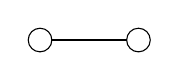
\begin{tikzpicture}
\draw (0,0) -- (1.25,0);
\draw[fill=white] (0,0) circle[radius=0.15];
\draw[fill=white] (1.25,0) circle[radius=0.15];
\end{tikzpicture}
\end{center}
We immediately see that we have two fundamental roots, i.e.\ $\Pi = \{\pi_1,\pi_2\}$, since there are two circles in the diagram. The bond number is $n_{12} = 1$, so the two fundamental roots have the same length. Moreover, by definition
\bse
1=n_{12} = C_{12}C_{21}
\ese
and since the off-diagonal entries of the Cartan matrix are non-positive integers, the only possibility is $C_{12}=C_{21}=-1$, so that we have
\bse
C = \biggl( \begin{matrix}2 & -1\\ -1 & 2\end{matrix}\biggr).
\ese
To determine the angle $\varphi$ between $\pi_1$ and $\pi_2$, recall that
\bse
1 = n_{12} = 4 \cos^2\varphi,
\ese
and hence $|\cos\varphi|=\frac{1}{2}$. There are two solutions, namely $\varphi=60^\circ$ and $\varphi=120^\circ$.
\begin{center}
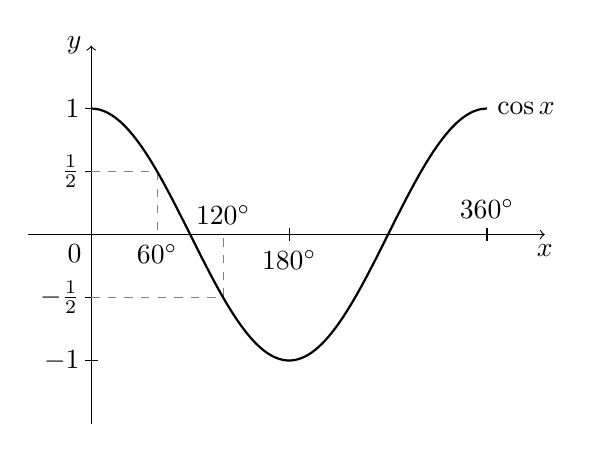
\begin{tikzpicture}[xscale=0.8,yscale=1.6]
\draw[->] (-1,0) -- (7.2,0) node[below] {$x$};
\draw[->] (0,-1.5) -- (0,1.5) node[left] {$y$};
\foreach \i/\j in {-2/-1,-1/-\frac{1}{2},1/\frac{1}{2},2/1} {
\draw (-0.1,0.5*\i) -- (0.1,0.5*\i) node[left=3pt] {$\j$};
}
\draw (0,0) node[below left] {$0$};
\draw[gray,dashed] (0,0.5) -| (pi/3,0);
\draw (pi/3,0) node[below] {$60^\circ$};
\draw[gray,dashed] (0,-0.5) -| (2*pi/3,0);
\draw (2*pi/3,0) node[above] {$120^\circ$};
\draw (pi,0.05) -- (pi,-0.05) node[below] {$180^\circ$};
\draw (2*pi,-0.05) -- (2*pi,0.05) node[above] {$360^\circ$};
\draw[thick,smooth,samples=100,variable=\x,domain=0:2*pi] plot(\x,{cos(deg(\x))}) node[right] {$\cos x$};
\end{tikzpicture}
\end{center}
By definition, we have
\bse
\cos \varphi = \frac{\kappa^*(\pi_1,\pi_2)}{|\pi_1|\,|\pi_2|},
\ese
and therefore
\bse
0 > C_{12} = 2\frac{\kappa^*(\pi_1,\pi_2)}{\kappa^*(\pi_1,\pi_1)} = 2\frac{|\pi_1|\,|\pi_2|\cos\varphi}{\kappa^*(\pi_1,\pi_1)} = 2\frac{|\pi_2|}{|\pi_1|}\cos\varphi.
\ese
It follows that $\cos\varphi<0$, and hence $\varphi = 120^\circ$. We can thus plot the two fundamental roots in a plane as follows.
\begin{center}
\begin{tikzpicture}[scale=2]
\draw[thin,lightgray] (-1.5,0) -- (1.5,0);
\draw[thin,lightgray] (0,-1.25) -- (0,1.25);
\draw[thick,->] (0,0) -- (1,0) node[above right] {$\pi_1$};
\draw[thick,->] (0,0) -- (cos 120,sin 120) node[above left] {$\pi_2$};
\end{tikzpicture}
\end{center}
We can determine all the other roots in $\Phi$ by repeated action of the Weyl group. For instance, we easily find that $s_{\pi_1}(\pi_1) = -\pi_1$ and $s_{\pi_2}(\pi_2) = -\pi_2$. We also have
\bse
s_{\pi_1}(\pi_2)  =  \pi_2-2\frac{\kappa^*(\pi_1,\pi_2)}{\kappa^*(\pi_1,\pi_1)}\pi_1 = \pi_2 -2 (-\tfrac{1}{2}) \pi_1 = \pi_1+\pi_2.
\ese
Finally, we have $s_{\pi_1+\pi_2}(\pi_1+\pi_2)=-(\pi_1+\pi_2)$.  Any further action by Weyl transformations simply permutes these roots. Hence, we have
\bse
\Phi=\{\pi_1,-\pi_1,\pi_2,-\pi_2,\pi_1+\pi_2,-(\pi_1+\pi_2)\}
\ese
and these are all the roots.
\begin{center}
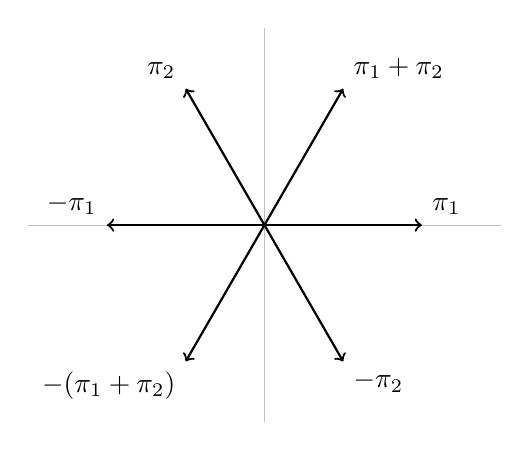
\begin{tikzpicture}[scale=2]
\draw[thin,lightgray] (-1.5,0) -- (1.5,0);
\draw[thin,lightgray] (0,-1.25) -- (0,1.25);
\draw[thick,->] (0,0) -- (1,0) node[above right] {$\pi_1$};
\draw[thick,->] (0,0) -- (cos 120,sin 120) node[above left] {$\pi_2$};
\draw[thick,->] (0,0) -- (-1,0) node[above left] {$-\pi_1$};
\draw[thick,->] (0,0) -- (-cos 120,-sin 120) node[below right] {$-\pi_2$};
\draw[thick,->] (0,0) -- (cos 60,sin 60) node[above right] {$\pi_1+\pi_2$};
\draw[thick,->] (0,0) -- (-cos 60,-sin 60) node[below left] {$-(\pi_1+\pi_2)$};
\end{tikzpicture}
\end{center}
Since $H^*=\lspan_\C(\Pi)$, we have $\dim H^*=2$, thus the dimension of the Cartan  subalgebra is also $2$. Since $|\Phi|=6$, we know that any Cartan-Weyl basis of the Lie algebra $A_2$ must have $2+6=8$ elements. Hence, the dimension of $A_2$ is 8. 

To complete our reconstruction of $A_2$, we would now like to understand how its bracket behaves. This amounts to finding its structure constants. Note that since $\dim A_2 = 8$, the structure constants $C^k_{\phantom{h}ij}$ consist of $8^3=512$ complex numbers (not all unrelated, of course).

Denote by $\{h_1,h_2,e_3,\ldots,e_8\}$ a Cartan-Weyl basis of $A_2$, so that $H=\lspan_\C(\{h_1,h_2\})$ and the $e_\alpha$ are eigenvectors of every $h\in H$.
Since $A_2$ is simple, $H$ is abelian and hence
\bse
[h_1,h_2] = 0 \quad \Rightarrow \quad C^k_{\phantom{k}12}=C^k_{\phantom{k}21} = 0, \quad \forall \, 1\leq k \leq 8.
\ese
To each $e_\alpha$, for $3\leq \alpha \leq 8$, there is an associated $\lambda_\alpha\in\Phi$ such that
\bse
\forall \, h \in H : \ \ad(h)e_\alpha = \lambda_\alpha(h) e_\alpha.
\ese
In particular, for the basis elements $h_1,h_2$,
\bi{rCl}
[h_1,e_\alpha] & = & \ad(h_1)e_\alpha = \lambda_\alpha(h_1) e_\alpha,\\
{[h_2,e_\alpha]} & = & \ad(h_2)e_\alpha = \lambda_\alpha(h_2) e_\alpha,
\ei
so that we have
\bi{rCl}
C^1_{\phantom{1}1\alpha}=C^2_{\phantom{2}1\alpha}=0, &\quad & C^\alpha_{\phantom{\alpha}1\alpha} = \lambda_\alpha(h_1) , \quad \forall \, 3\leq \alpha \leq 8,\\
C^1_{\phantom{1}2\alpha}=C^2_{\phantom{2}2\alpha}=0, &\quad & C^\alpha_{\phantom{\alpha}2\alpha} = \lambda_\alpha(h_2) , \quad \forall \, 3\leq \alpha \leq 8.
\ei
Finally, we need to determine $[e_\alpha,e_\beta]$. By using the Jacobi identity, we have
\bi{rCl}
[h_i,[e_\alpha,e_\beta]] & = & - [e_\alpha,[e_\beta,h_i]] -[e_\beta,[h_i,e_\alpha]] \\
& = & - [e_\alpha,-\lambda_\beta(h_i)e_\beta] -[e_\beta,\lambda_\alpha(h_i)e_\alpha] \\
& = & \lambda_\beta(h_i) [e_\alpha,e_\beta] +\lambda_\alpha(h_i)[e_\alpha,e_\beta]\\
& = & (\lambda_\alpha(h_i)+\lambda_\beta(h_i) )[e_\alpha,e_\beta]  ,
\ei
that is,
\bse
\ad(h_i)[e_\alpha,e_\beta] =  (\lambda_\alpha(h_i)+\lambda_\beta(h_i) )[e_\alpha,e_\beta].
\ese

If $\lambda_\alpha+\lambda_\beta\in\Phi$, we have $[e_\alpha,e_\beta]=\xi e_\gamma$ for some $3\leq \gamma \leq 8$ and $\xi \in \C$. Let us label the roots in our previous plot as
\begin{center}
\def\arraystretch{1.25}
\setlength\tabcolsep{10pt}
\begin{tabular}{c|c|c|c|c|c}
$\lambda_3$ & $\lambda_4$ & $\lambda_5$ & $\lambda_6$ & $\lambda_7$ & $\lambda_8$\\
\hline
$\pi_1$ & $\pi_2$ & $\pi_1+\pi_2$ & $-\pi_1$ & $-\pi_2$ & $-(\pi_1+\pi_2)$ 
\end{tabular}
\end{center}
Then, for example
\bse
\ad(h)[e_3,e_4] = (\pi_1+\pi_2)(h) [e_3,e_4],
\ese
and hence $[e_3,e_4]$ is an eigenvector of $\ad(h)$ with eigenvalues $(\pi_1+\pi_2)(h)$. But so is $e_5$! Hence, we must have $[e_3,e_4]=\xi e_5$ for some $\xi \in \C$. Similarly, $[e_5,e_7]=\xi e_3$, and so on.

If $\lambda_\alpha+\lambda_\beta\notin\Phi$, then in order for the equation above to hold, we must have either $[e_\alpha,e_\beta]=0$ (so both sides are zero), or $\lambda_\alpha(h)+\lambda_\beta(h)=0$ for all $h$, i.e.\ $\lambda_\alpha+\lambda_\beta=0$ as a functional. In the latter case, we must have $[e_\alpha,e_\beta]\in H$. This follows from a stronger version of the maximality property of the Cartan subalgebra $H$ of a simple Lie algebra $L$, namely that
\bse
\big(\forall \, h \in H : [h,x] = 0 \big)  \Rightarrow x\in H.
\ese
Summarising, we have
\bse
[e_\alpha,e_\beta] =
\begin{cases}
\xi e_\gamma & \text{if } \lambda_\alpha+\lambda_\beta\in\Phi\\
\in H & \text{if } \lambda_\alpha+\lambda_\beta=0\\
0 & \text{otherwise }
\end{cases}
\ese
and these relations con be used to determine the remaining structure constants of $A_2$.